% Supplementary Information. Generated by scripts/make_supplement.py; do not edit by hand.
\documentclass[10pt]{article}
\usepackage[a4paper,margin=2cm,landscape]{geometry}
\usepackage{booktabs,graphicx,caption,xcolor,amssymb,float}
\usepackage[T1]{fontenc}
\usepackage{helvet}\renewcommand{\familydefault}{\sfdefault}
\usepackage{courier}\usepackage[hidelinks]{hyperref}
\graphicspath{{../docs/figures/}}
\captionsetup{labelformat=empty,justification=raggedright,singlelinecheck=false}
\newcommand{\todo}[1]{\textcolor{red}{[TODO: #1]}}
% generated by scripts/make_supplement.py: S-numbers used in the main text
\newcommand{\STqc}{S1}
\newcommand{\STmethods}{S2}
\newcommand{\STari}{S3}
\newcommand{\STnmi}{S4}
\newcommand{\STstats}{S5}
\newcommand{\STstatsrob}{S6}
\newcommand{\STstatsrunner}{S7}
\newcommand{\STranks}{S8}
\newcommand{\STseeds}{S9}
\newcommand{\STlottery}{S10}
\newcommand{\STmclust}{S11}
\newcommand{\STgain}{S12}
\newcommand{\STmetrics}{S13}
\newcommand{\STres}{S14}
\newcommand{\STagree}{S15}
\newcommand{\STk}{S16}
\newcommand{\STbrca}{S17}
\newcommand{\SThistar}{S18}
\newcommand{\STepoch}{S19}
\newcommand{\STaudit}{S20}
\newcommand{\STinv}{S21}
\newcommand{\STcov}{S22}
\newcommand{\SFlottery}{S1}
\newcommand{\SFsens}{S2}
\newcommand{\SFboundary}{S3}
\newcommand{\SNdata}{1}
\newcommand{\SNmethods}{2}
\newcommand{\SNmetrics}{3}
\newcommand{\SNstats}{4}
\newcommand{\SNaudit}{5}
\newcommand{\SNcompute}{6}

\begin{document}
\begin{center}{\Large\bfseries Supplementary Information}\\[4pt]
Benchmarking the accuracy, robustness and reproducibility of spatial domain identification methods\end{center}
\section*{Supplementary Notes}
\subsection*{Supplementary Note 1. Data and preprocessing}
DLPFC count matrices from spatialLIBD and layer annotations from the SEDR analyses repository; STARmap and MERFISH matrices and annotations from the BASS analyses. Genes in fewer than 50 spots or with fewer than 10 counts were removed for Visium; counts were normalised to the library size, log-transformed and reduced to 2000 highly variable genes (Visium) or all panel genes, then scaled and reduced by PCA (200 components for Visium, 50 for panels). Sections, splits and label provenance are listed in configs/datasets.yaml; per-section statistics are in Supplementary Table~\STqc.

\subsection*{Supplementary Note 2. Methods and settings}
Every method was run from its official code with the settings of its tutorial or paper (Supplementary Table~\STmethods). The true number of domains was given to every method. Neighbourhood radii given in pixels were converted to multiples of the spot or cell spacing so that they transfer across technologies. Methods that output an embedding were additionally clustered with a 20-start tied-covariance Gaussian mixture keeping the best likelihood.

\subsection*{Supplementary Note 3. Metrics}
Agreement: ARI, NMI, AMI. Per-domain: clusters matched to domains with the Hungarian algorithm; macro-F1, missed domains, recall of domains below 5\% of spots. Spatial: CHAOS (mean distance to the nearest same-cluster neighbour), PAS (fraction of spots whose cluster differs from most of their ten neighbours), Moran's I of the labels, boundary F1. Label-free: silhouette, Davies--Bouldin, Calinski--Harabasz. Definitions and code: spatialbench/metrics.py (unit tests in tests/).

\subsection*{Supplementary Note 4. Statistics}
Sections are nested in clusters (three DLPFC donors, STARmap, MERFISH). Differences to the reference are equal-weight means of cluster means with 95\% percentile intervals from a hierarchical bootstrap (5000 resamples: clusters, then sections within clusters). Equivalence: 90\% interval within $\pm$0.03 ARI, a margin fixed before the analysis. Ranks and the probability of ranking first come from the same resamples. The reference method was chosen after seeing the means, so these comparisons are exploratory. Code: \texttt{scripts/stats\_cluster\_aware.py}.

\subsection*{Supplementary Note 5. Audit of released code}
Repositories were screened with \texttt{scripts/audit\_leakage.py} for six patterns of label use (Supplementary Table~\STaudit), and every candidate line was read by one author. The taxonomy and all judgements, including false alarms, are in \texttt{docs/LEAKAGE\_AUDIT.md}. The authors of the methods concerned have not yet been contacted.

\subsection*{Supplementary Note 6. Computing environment}
All runs used one CPU thread per job on a 4-core Intel Xeon (2.8 GHz) with 15 GB of memory, Python 3.13, R 4.3.3 and mclust 6.0.1. Memory-heavy methods (DeepST, BayesSpace, NichePCA) were run one job at a time.

\clearpage\section*{Supplementary Tables}
\begin{table}[!htbp]\centering
\caption*{\textbf{Supplementary Table S1.} Data and quality control per section. Sparsity: fraction of zero entries. Annotated: fraction of spots or cells with a domain label. Smallest domain: fraction of annotated spots in the smallest domain. Imbalance: largest over smallest domain size.}
\scriptsize
\begin{tabular}{lrrrrrrrr}
\toprule
Section & Spots/cells & Genes & Median counts & Sparsity & Annotated & Domains & Smallest domain & Imbalance \\
\midrule
DLPFC 151507 & 4226 & 33538 & 2464 & 0.96 & 1.00 & 7 & 0.072 & 4.0 \\
DLPFC 151508 & 4384 & 33538 & 2019 & 0.96 & 1.00 & 7 & 0.046 & 6.9 \\
DLPFC 151509 & 4789 & 33538 & 2416 & 0.96 & 1.00 & 7 & 0.035 & 11.3 \\
DLPFC 151510 & 4634 & 33538 & 2319 & 0.96 & 0.99 & 7 & 0.039 & 9.9 \\
DLPFC 151669 & 3661 & 33538 & 3470 & 0.95 & 0.99 & 5 & 0.063 & 9.3 \\
DLPFC 151670 & 3498 & 33538 & 3113 & 0.95 & 1.00 & 5 & 0.060 & 10.4 \\
DLPFC 151671 & 4110 & 33538 & 3743 & 0.94 & 1.00 & 5 & 0.060 & 7.8 \\
DLPFC 151672 & 4015 & 33538 & 3482 & 0.95 & 0.97 & 5 & 0.078 & 5.2 \\
DLPFC 151673 & 3639 & 33538 & 4120 & 0.93 & 0.99 & 7 & 0.060 & 4.5 \\
DLPFC 151674 & 3673 & 33538 & 5334 & 0.92 & 0.99 & 7 & 0.062 & 4.1 \\
DLPFC 151675 & 3592 & 33538 & 3140 & 0.95 & 0.99 & 7 & 0.077 & 2.8 \\
DLPFC 151676 & 3460 & 33538 & 3419 & 0.94 & 0.99 & 7 & 0.074 & 3.3 \\
STARmap 20180417\_BZ5\_control & 1049 & 166 & 604 & 0.69 & 1.00 & 4 & 0.082 & 5.2 \\
STARmap 20180419\_BZ9\_control & 1053 & 166 & 301 & 0.77 & 1.00 & 4 & 0.078 & 6.1 \\
STARmap 20180424\_BZ14\_control & 1088 & 166 & 393 & 0.70 & 1.00 & 4 & 0.031 & 13.6 \\
MERFISH -0.04 & 5488 & 155 & 241 & 0.58 & 1.00 & 8 & 0.019 & 13.1 \\
MERFISH -0.09 & 5557 & 155 & 260 & 0.57 & 1.00 & 8 & 0.025 & 9.7 \\
MERFISH -0.14 & 5926 & 155 & 246 & 0.57 & 1.00 & 8 & 0.036 & 7.8 \\
MERFISH -0.19 & 5803 & 155 & 254 & 0.58 & 1.00 & 8 & 0.043 & 5.6 \\
MERFISH -0.24 & 5543 & 155 & 244 & 0.59 & 1.00 & 8 & 0.041 & 7.0 \\
Breast block\_a\_1 & 3798 & 36601 & 20762 & 0.85 & 1.00 & 20 & 0.007 & 16.0 \\
Stereo-seq E9.5\_E1S1 & 5913 & 25568 & 14039 & 0.86 & 1.00 & 12 & 0.017 & 15.5 \\
Stereo-seq E10.5\_E2S1 & 8494 & 22385 & 7102 & 0.91 & 1.00 & 18 & 0.013 & 13.1 \\
Stereo-seq E10.5\_E1S1 & 18408 & 25201 & 11786 & 0.86 & 1.00 & 13 & 0.011 & 23.5 \\
\bottomrule
\end{tabular}

\end{table}

\begin{table}[!htbp]\centering
\caption*{\textbf{Supplementary Table S2.} Benchmarked methods: code source, version, settings source, clustering and every deviation from the published tutorial (from configs/methods.yaml).}
\scriptsize
\begin{tabular}{p{1.6cm}p{2.0cm}p{3.0cm}p{1.2cm}p{1.2cm}p{2.2cm}p{5.2cm}}
\toprule
Method & Type & Code & Commit & Settings & Default clustering & Deviations from the tutorial \\
\midrule
HiSTaR & deep graph VAE & PyTorch port of the official code (hicast/histar.py) & 0039a3b & paper & 3-start Gaussian mixture (scikit-learn, tied) & \parbox[t]{5.2cm}{\raggedright masking at inference removed in 'deterministic' variant only; headline uses published behaviour; per-section lambda\_sim tuning described in the paper's supplement is NOT applied} \\
GraphST & deep graph contrastive autoencoder & pip GraphST 1.1.1; tutorials from JinmiaoChenLab/GraphST & d62b0b7 & tutorial & R mclust EEE on 20 PCs of the embedding & \parbox[t]{5.2cm}{\raggedright reported with and without the tutorial's label refinement (graphst vs graphst\_refined)} \\
BANKSY & neighbourhood-augmented features (non-deep) & pip pybanksy 1.3.5 & 9278996 & tutorial & 3-start Gaussian mixture (scikit-learn, tied) & \parbox[t]{5.2cm}{\raggedright both recommended lambdas are run: 0.2 (cell typing) and 0.8 (domain segmentation)} \\
SpaGCN & graph convolutional network & pip SpaGCN 1.2.7 & dc7a1c2 & tutorial & iterative DEC clustering (own) & \parbox[t]{5.2cm}{\raggedright no histology image used (not available for all sections); reported with and without the hexagonal refinement} \\
STAGATE & deep graph attention autoencoder & QIFEIDKN/STAGATE\_pyG, installed from the clone & ae1158c & tutorial & R mclust EEE & \parbox[t]{5.2cm}{\raggedright radius expressed in spot spacings because our coordinates are on another scale (gives 5.8 neighbours per spot, as in the tutorial); torch\_sparse replaced by a stub only if the compiled extension is unavailable (it was compiled from source here)} \\
SEDR & deep masked graph autoencoder & JinmiaoChenLab/SEDR, installed from the clone & ef48360 & tutorial & R mclust EEE (seed 2023) & \parbox[t]{5.2cm}{\raggedright mclust called as SEDR.mclust\_R does, without its line that hard-codes the authors' R\_HOME (breaks R's LAPACK in a running session)} \\
SpaceFlow & deep graph infomax with spatial regularisation & pip SpaceFlow 1.0.4 & 58d1ab0 & package default & Leiden at a fixed resolution & \parbox[t]{5.2cm}{\raggedright networkx>=3 alias for removed to\_scipy\_sparse\_matrix; all-zero genes removed (cell\_ranger HVG binning fails on them with pandas 3)} \\
NichePCA & training-free (neighbour aggregation + PCA) & pip nichepca 0.1.0 & package 0.1.0 & package default & Leiden & \parbox[t]{5.2cm}{\raggedright } \\
CCST & deep graph infomax (4 GCN layers) & xiaoyeye/CCST, re-implemented in scripts/new\_methods.py bec & 890de27 & tutorial & k-means (n\_init=100) & \parbox[t]{5.2cm}{\raggedright graph threshold chosen to give about 6 neighbours per cell (the authors hand-pick a threshold per dataset)} \\
Spatial-MGCN & deep multi-view graph convolution & cs-wangbo/Spatial-MGCN, repository modules used directly & cf4412d & tutorial & k-means each epoch; epoch chosen by ARI against the annotation (LEAKAGE, see docs/LEAKAGE\_AUDIT.md) & \parbox[t]{5.2cm}{\raggedright unannotated spots kept (the released script deletes them before training); label-free epoch rule} \\
DeepST & deep graph + augmentation (no histology) & JiangBioLab/DeepST (deepstkit), used from the clone & e37997f & tutorial & Leiden at the given K + spatial refinement & \parbox[t]{5.2cm}{\raggedright no histology features; memory-heavy: run one job at a time} \\
BASS & Bayesian hierarchical model & zhengli09/BASS, installed from the clone & 5c2690f & tutorial & own (joint cell-type and domain model) & \parbox[t]{5.2cm}{\raggedright each section analysed separately (the authors' MERFISH/DLPFC analyses are multi-sample)} \\
BayesSpace & Bayesian statistical model & edward130603/BayesSpace tag v1.5.1 (older release; newer one & ba8b422 & package default & own MCMC & \parbox[t]{5.2cm}{\raggedright Visium only (needs a hexagonal spot lattice)} \\
Linear diffusion & training-free &  &  & fixed rule & 3-start Gaussian mixture (scikit-learn, tied) & \parbox[t]{5.2cm}{\raggedright settings fixed on DLPFC donor 1 before any other data were analysed} \\
AnisoST & training-free, edge-preserving diffusion &  &  & fixed rule & 3-start Gaussian mixture (scikit-learn, tied) & \parbox[t]{5.2cm}{\raggedright same as linear\_diffusion} \\
PCA & training-free &  &  & fixed rule & 3-start Gaussian mixture (scikit-learn, tied) & \parbox[t]{5.2cm}{\raggedright } \\
\bottomrule
\end{tabular}

\end{table}

\begin{table}[!htbp]\centering
\caption*{\textbf{Supplementary Table S3.} Mean ARI over sections and seeds per dataset with each method's own clustering and with the 20-start best-likelihood Gaussian mixture on its embedding. Training-free baselines are clustered only with the 20-start mixture. Methods that cluster internally have no 20-start value.}
\footnotesize
\begin{tabular}{lrrrrrr}
\toprule
Method & DLPFC own & DLPFC 20-start & STARmap own & STARmap 20-start & MERFISH own & MERFISH 20-start \\
\midrule
Linear diffusion & -- & 0.558 & -- & 0.705 & -- & 0.497 \\
AnisoST & 0.526 & 0.551 & 0.564 & 0.622 & 0.377 & 0.363 \\
PCA & -- & 0.409 & -- & 0.294 & -- & 0.130 \\
HiSTaR & 0.491 & 0.544 & 0.593 & 0.658 & 0.221 & 0.264 \\
GraphST & 0.514 & 0.531 & 0.388 & 0.484 & 0.251 & 0.254 \\
BANKSY $\lambda$=0.8 & 0.494 & 0.518 & 0.740 & 0.694 & 0.428 & 0.410 \\
BANKSY $\lambda$=0.2 & 0.514 & 0.518 & 0.502 & 0.529 & 0.211 & 0.222 \\
SpaGCN & 0.422 & -- & 0.267 & -- & 0.151 & -- \\
STAGATE & 0.497 & 0.548 & 0.479 & 0.572 & 0.368 & 0.342 \\
SEDR & 0.515 & 0.551 & 0.593 & 0.236 & 0.406 & 0.167 \\
SpaceFlow & 0.312 & 0.326 & 0.628 & 0.668 & 0.389 & 0.260 \\
NichePCA & 0.321 & 0.506 & 0.692 & 0.604 & 0.475 & 0.403 \\
CCST & 0.437 & 0.359 & 0.505 & 0.435 & 0.212 & 0.157 \\
Spatial-MGCN & 0.418 & 0.391 & 0.303 & 0.245 & 0.182 & 0.133 \\
DeepST & 0.459 & 0.435 & 0.368 & 0.409 & 0.231 & 0.163 \\
BASS & 0.484 & -- & 0.716 & -- & 0.582 & -- \\
BayesSpace & 0.437 & -- & -- & -- & -- & -- \\
\bottomrule
\end{tabular}

\end{table}

\begin{table}[!htbp]\centering
\caption*{\textbf{Supplementary Table S4.} As Supplementary Table~\STari{} for normalised mutual information (NMI).}
\footnotesize
\begin{tabular}{lrrrrrr}
\toprule
Method & DLPFC default & DLPFC matched & STARmap default & STARmap matched & MERFISH default & MERFISH matched \\
\midrule
Linear diffusion & 0.668 & 0.676 & 0.700 & 0.699 & 0.602 & 0.614 \\
AnisoST & 0.653 & 0.665 & 0.582 & 0.590 & 0.494 & 0.488 \\
PCA & 0.497 & 0.506 & 0.301 & 0.326 & 0.227 & 0.216 \\
HiSTaR & 0.637 & 0.660 & 0.602 & 0.653 & 0.375 & 0.405 \\
GraphST & 0.621 & 0.634 & 0.435 & 0.481 & 0.408 & 0.404 \\
BANKSY $\lambda$=0.8 & 0.605 & 0.611 & 0.713 & 0.680 & 0.567 & 0.558 \\
BANKSY $\lambda$=0.2 & 0.610 & 0.611 & 0.530 & 0.535 & 0.302 & 0.318 \\
SpaGCN & 0.555 & 0.555 & 0.317 & 0.317 & 0.238 & 0.238 \\
STAGATE & 0.641 & 0.668 & 0.492 & 0.552 & 0.490 & 0.473 \\
SEDR & 0.654 & 0.654 & 0.614 & 0.303 & 0.544 & 0.312 \\
SpaceFlow & 0.456 & 0.480 & 0.640 & 0.655 & 0.509 & 0.441 \\
NichePCA & 0.460 & 0.629 & 0.703 & 0.604 & 0.567 & 0.540 \\
CCST & 0.576 & 0.511 & 0.453 & 0.421 & 0.334 & 0.314 \\
Spatial-MGCN & 0.599 & 0.581 & 0.307 & 0.271 & 0.265 & 0.232 \\
DeepST & 0.628 & 0.572 & 0.489 & 0.429 & 0.370 & 0.261 \\
BASS & 0.639 & 0.639 & 0.690 & 0.690 & 0.638 & 0.638 \\
BayesSpace & 0.597 & 0.597 & -- & -- & -- & -- \\
\bottomrule
\end{tabular}

\end{table}

\begin{table}[!htbp]\centering
\caption*{\textbf{Supplementary Table S5.} Difference in mean ARI between linear diffusion and each method (own clustering), equal-weight mean of cluster means; 95\% interval from a hierarchical bootstrap over five clusters (three DLPFC donors, STARmap, MERFISH). Test only: the same estimate without the development sections. Verdict: baseline higher if the interval is above zero; unresolved otherwise; no comparison met the equivalence criterion (90\% interval within $\pm$0.03).}
\scriptsize
\begin{tabular}{lrrrrrrrl}
\toprule
Method & $\Delta$ & 95\% CI & DLPFC & STARmap & MERFISH & Test only & 95\% CI & Verdict \\
\midrule
PCA & +0.245 & (+0.140, +0.361) & +0.15 & +0.41 & +0.37 & +0.262 & (+0.140, +0.388) & baseline higher \\
SpaGCN & +0.238 & (+0.127, +0.362) & +0.14 & +0.44 & +0.35 & +0.269 & (+0.146, +0.400) & baseline higher \\
Spatial-MGCN & +0.227 & (+0.132, +0.337) & +0.14 & +0.40 & +0.32 & +0.253 & (+0.151, +0.381) & baseline higher \\
SpaceFlow & +0.185 & (+0.101, +0.278) & +0.25 & +0.08 & +0.11 & +0.194 & (+0.098, +0.296) & baseline higher \\
DeepST & +0.180 & (+0.073, +0.286) & +0.10 & +0.34 & +0.27 & +0.213 & (+0.084, +0.330) & baseline higher \\
CCST & +0.170 & (+0.096, +0.242) & +0.12 & +0.20 & +0.28 & +0.157 & (+0.071, +0.252) & baseline higher \\
NichePCA & +0.149 & (+0.040, +0.249) & +0.24 & +0.01 & +0.02 & +0.116 & (-0.032, +0.263) & baseline higher \\
GraphST & +0.139 & (+0.029, +0.253) & +0.04 & +0.32 & +0.25 & +0.148 & (+0.021, +0.279) & baseline higher \\
BANKSY $\lambda$=0.2 & +0.124 & (+0.029, +0.228) & +0.04 & +0.20 & +0.29 & +0.127 & (+0.040, +0.234) & baseline higher \\
BayesSpace & +0.121 & (+0.038, +0.213) & +0.12 & -- & -- & +0.141 & (+0.027, +0.246) & baseline higher \\
HiSTaR & +0.118 & (+0.024, +0.217) & +0.07 & +0.11 & +0.28 & +0.119 & (-0.018, +0.246) & baseline higher \\
STAGATE & +0.108 & (+0.025, +0.193) & +0.06 & +0.23 & +0.13 & +0.117 & (+0.042, +0.179) & baseline higher \\
AnisoST & +0.071 & (+0.019, +0.129) & +0.03 & +0.14 & +0.12 & +0.077 & (+0.033, +0.127) & baseline higher \\
SEDR & +0.066 & (+0.012, +0.130) & +0.04 & +0.11 & +0.09 & +0.058 & (+0.002, +0.122) & baseline higher \\
BANKSY $\lambda$=0.8 & +0.045 & (-0.008, +0.091) & +0.06 & -0.04 & +0.07 & +0.041 & (-0.039, +0.107) & unresolved \\
BASS & +0.025 & (-0.046, +0.101) & +0.07 & -0.01 & -0.09 & +0.015 & (-0.068, +0.107) & unresolved \\
\bottomrule
\end{tabular}

\end{table}

\begin{table}[!htbp]\centering
\caption*{\textbf{Supplementary Table S6.} As Supplementary Table~\STstats{} with the 20-start best-likelihood clustering applied to each embedding.}
\scriptsize
\begin{tabular}{lrrrrrrrl}
\toprule
Method & $\Delta$ & 95\% CI & DLPFC & STARmap & MERFISH & Test only & 95\% CI & Verdict \\
\midrule
Spatial-MGCN & +0.265 & (+0.137, +0.406) & +0.17 & +0.46 & +0.36 & +0.309 & (+0.187, +0.448) & baseline higher \\
PCA & +0.245 & (+0.140, +0.359) & +0.15 & +0.41 & +0.37 & +0.262 & (+0.142, +0.385) & baseline higher \\
CCST & +0.242 & (+0.142, +0.324) & +0.20 & +0.27 & +0.34 & +0.250 & (+0.126, +0.353) & baseline higher \\
SpaGCN & +0.238 & (+0.124, +0.366) & +0.14 & +0.44 & +0.35 & +0.269 & (+0.141, +0.404) & baseline higher \\
DeepST & +0.200 & (+0.102, +0.297) & +0.12 & +0.30 & +0.33 & +0.202 & (+0.088, +0.315) & baseline higher \\
SpaceFlow & +0.194 & (+0.097, +0.269) & +0.23 & +0.04 & +0.24 & +0.202 & (+0.060, +0.289) & baseline higher \\
SEDR & +0.164 & (-0.007, +0.352) & +0.01 & +0.47 & +0.33 & +0.199 & (-0.028, +0.415) & unresolved \\
BayesSpace & +0.121 & (+0.037, +0.207) & +0.12 & -- & -- & +0.141 & (+0.035, +0.249) & baseline higher \\
BANKSY $\lambda$=0.2 & +0.114 & (+0.014, +0.225) & +0.04 & +0.18 & +0.28 & +0.112 & (+0.008, +0.230) & baseline higher \\
GraphST & +0.109 & (+0.010, +0.209) & +0.03 & +0.22 & +0.24 & +0.101 & (-0.006, +0.210) & baseline higher \\
NichePCA & +0.070 & (+0.017, +0.127) & +0.05 & +0.10 & +0.09 & +0.066 & (+0.014, +0.125) & baseline higher \\
HiSTaR & +0.064 & (-0.018, +0.163) & +0.01 & +0.05 & +0.23 & +0.066 & (-0.056, +0.197) & unresolved \\
STAGATE & +0.064 & (+0.000, +0.133) & +0.01 & +0.13 & +0.15 & +0.073 & (+0.014, +0.137) & baseline higher \\
AnisoST & +0.048 & (-0.007, +0.105) & +0.01 & +0.08 & +0.13 & +0.058 & (+0.005, +0.127) & unresolved \\
BANKSY $\lambda$=0.8 & +0.044 & (-0.007, +0.095) & +0.04 & +0.01 & +0.09 & +0.054 & (-0.009, +0.117) & unresolved \\
BASS & +0.025 & (-0.044, +0.101) & +0.07 & -0.01 & -0.09 & +0.015 & (-0.072, +0.109) & unresolved \\
\bottomrule
\end{tabular}

\end{table}

\begin{table}[!htbp]\centering
\caption*{\textbf{Supplementary Table S7.} Rank of each method (own clustering) in the hierarchical bootstrap.}
\footnotesize
\begin{tabular}{lrrrrrr}
\toprule
Method & P(rank 1) & Median rank & 95\% interval & P(rank 1), default & Median rank, default & 95\% interval, default \\
\midrule
Linear diffusion & 0.60 & 1 & 1--3 & 0.56 & 1 & 1--3 \\
BASS & 0.25 & 2 & 1--10 & 0.35 & 2 & 1--9 \\
BANKSY $\lambda$=0.8 & 0.02 & 3 & 2--9 & 0.06 & 3 & 1--9 \\
AnisoST & 0.03 & 4 & 1--7 & 0.00 & 5 & 2--7 \\
HiSTaR & 0.06 & 6 & 1--8 & 0.00 & 8 & 3--11 \\
STAGATE & 0.01 & 6 & 2--8 & 0.01 & 7 & 3--11 \\
NichePCA & 0.00 & 6 & 3--10 & 0.00 & 10 & 4--16 \\
GraphST & 0.00 & 8 & 4--10 & 0.01 & 9 & 3--12 \\
BANKSY $\lambda$=0.2 & 0.00 & 9 & 4--10 & 0.01 & 8 & 3--12 \\
SEDR & 0.03 & 10 & 1--15 & 0.01 & 4 & 2--6 \\
DeepST & 0.00 & 11 & 11--14 & 0.00 & 12 & 8--13 \\
SpaceFlow & 0.00 & 12 & 7--16 & 0.00 & 12 & 6--16 \\
SpaGCN & 0.00 & 14 & 11--16 & 0.00 & 15 & 11--16 \\
CCST & 0.00 & 14 & 11--16 & 0.00 & 11 & 8--14 \\
PCA & 0.00 & 14 & 11--16 & 0.00 & 16 & 13--16 \\
Spatial-MGCN & 0.00 & 15 & 12--16 & 0.00 & 14 & 11--15 \\
\bottomrule
\end{tabular}

\end{table}

\begin{table}[!htbp]\centering
\caption*{\textbf{Supplementary Table S8.} Seed-to-seed standard deviation of ARI (mean over sections; own clustering, or 20-start clustering for the baselines). Methods run with one seed have no value.}
\footnotesize
\begin{tabular}{lrrrr}
\toprule
Method & DLPFC & STARmap & MERFISH & Seeds (D/S/M) \\
\midrule
Linear diffusion & 0.039 & 0.012 & 0.054 & 3/3/3 \\
AnisoST & 0.022 & 0.042 & 0.015 & 3/3/3 \\
PCA & 0.015 & 0.019 & 0.015 & 3/3/3 \\
HiSTaR & 0.047 & 0.180 & 0.053 & 3/3/3 \\
GraphST & -- & 0.086 & 0.031 & 1/3/3 \\
BANKSY $\lambda$=0.8 & 0.067 & 0.006 & 0.041 & 3/3/3 \\
BANKSY $\lambda$=0.2 & 0.056 & 0.063 & 0.022 & 3/3/3 \\
SpaGCN & 0.038 & 0.030 & 0.016 & 3/3/3 \\
STAGATE & -- & -- & -- & 1/1/1 \\
SEDR & 0.042 & 0.083 & 0.060 & 3/3/3 \\
SpaceFlow & 0.032 & 0.101 & 0.030 & 3/3/3 \\
NichePCA & 0.023 & 0.034 & 0.029 & 3/3/3 \\
CCST & -- & -- & -- & 1/1/1 \\
Spatial-MGCN & -- & -- & -- & 1/1/1 \\
DeepST & 0.042 & 0.030 & 0.028 & 3/3/3 \\
BASS & -- & -- & -- & 1/1/1 \\
BayesSpace & -- & -- & -- & 1/0/0 \\
\bottomrule
\end{tabular}

\end{table}

\begin{table}[!htbp]\centering
\caption*{\textbf{Supplementary Table S9.} Clustering one fixed embedding per section 20 times with a single-start Gaussian mixture (20 sections per method). Range and SD of ARI across the 20 fits; best minus mean: ARI gain of choosing the best fit by agreement with the labels; best-likelihood minus mean: gain of choosing the fit with the highest likelihood; $\rho$: median Spearman correlation between log-likelihood and ARI.}
\scriptsize
\begin{tabular}{lrrrrrrrr}
\toprule
Method & Median range & IQR & Mean SD & Best-by-ARI minus mean & Best-likelihood minus mean & $\rho$ DLPFC & $\rho$ STARmap & $\rho$ MERFISH \\
\midrule
SpaceFlow & 0.07 & 0.05--0.11 & 0.028 & 0.036 & +0.005 & -0.05 & +0.60 & +0.51 \\
GraphST & 0.07 & 0.02--0.14 & 0.031 & 0.044 & +0.017 & +0.36 & +0.23 & -0.04 \\
Spatial-MGCN & 0.12 & 0.08--0.15 & 0.033 & 0.048 & -0.017 & +0.07 & +0.12 & +0.19 \\
DeepST & 0.12 & 0.08--0.24 & 0.046 & 0.063 & -0.016 & +0.14 & +0.38 & -0.26 \\
PCA & 0.15 & 0.08--0.22 & 0.039 & 0.055 & +0.020 & -0.16 & +0.17 & -0.25 \\
SEDR & 0.17 & 0.10--0.24 & 0.060 & 0.099 & +0.038 & +0.50 & -0.64 & -0.20 \\
CCST & 0.17 & 0.08--0.29 & 0.060 & 0.076 & -0.062 & -0.04 & +0.26 & -0.17 \\
AnisoST & 0.17 & 0.14--0.26 & 0.060 & 0.091 & +0.039 & +0.48 & +0.47 & -0.36 \\
STAGATE & 0.18 & 0.12--0.23 & 0.053 & 0.070 & +0.041 & +0.62 & +0.57 & -0.22 \\
HiSTaR & 0.19 & 0.14--0.25 & 0.068 & 0.113 & +0.069 & +0.22 & +0.53 & -0.57 \\
Linear diffusion & 0.19 & 0.16--0.26 & 0.064 & 0.078 & +0.060 & +0.88 & +0.26 & -0.01 \\
NichePCA & 0.21 & 0.16--0.28 & 0.067 & 0.095 & +0.037 & +0.65 & +0.54 & +0.22 \\
BANKSY $\lambda$=0.2 & 0.22 & 0.13--0.31 & 0.064 & 0.098 & +0.043 & +0.25 & +0.57 & +0.10 \\
BANKSY $\lambda$=0.8 & 0.22 & 0.18--0.29 & 0.080 & 0.100 & +0.008 & +0.19 & +0.76 & -0.08 \\
\bottomrule
\end{tabular}

\end{table}

\begin{table}[!htbp]\centering
\caption*{\textbf{Supplementary Table S10.} R mclust (EEE, default initialisation) on the same embedding after random permutation of the spot order or adding Gaussian noise at 1\% of each feature's standard deviation (10 repetitions each). Range: median over sections of the ARI range; runs $>$0.05: share of perturbations that changed ARI by more than 0.05 from the unperturbed fit.}
\footnotesize
\begin{tabular}{lrrrrrr}
\toprule
Method & Embeddings & Seed range (mean) & Seed range (max) & Range $>$0.1 & Noise range, full init. & Full minus seeded mean \\
\midrule
Linear diffusion & 20 & 0.19 & 0.35 & 88\% & 0.14 & -0.001 \\
NichePCA & 20 & 0.18 & 0.42 & 82\% & 0.18 & +0.004 \\
PCA & 20 & 0.16 & 0.46 & 65\% & 0.12 & -0.023 \\
BANKSY $\lambda$=0.8 & 20 & 0.15 & 0.34 & 65\% & 0.11 & -0.005 \\
SEDR & 20 & 0.14 & 0.33 & 71\% & 0.08 & +0.003 \\
STAGATE & 20 & 0.13 & 0.27 & 65\% & 0.09 & +0.019 \\
HiSTaR & 20 & 0.12 & 0.32 & 59\% & 0.09 & -0.004 \\
AnisoST & 20 & 0.11 & 0.22 & 53\% & 0.06 & -0.034 \\
Spatial-MGCN & 20 & 0.10 & 0.40 & 41\% & 0.06 & +0.011 \\
BANKSY $\lambda$=0.2 & 20 & 0.10 & 0.28 & 53\% & 0.07 & -0.004 \\
SpaceFlow & 20 & 0.10 & 0.20 & 47\% & 0.08 & -0.001 \\
CCST & 20 & 0.09 & 0.35 & 24\% & 0.07 & +0.012 \\
GraphST & 20 & 0.09 & 0.26 & 41\% & 0.07 & -0.006 \\
DeepST & 20 & 0.06 & 0.17 & 24\% & 0.03 & +0.009 \\
\bottomrule
\end{tabular}

\end{table}

\begin{table}[!htbp]\centering
\caption*{\textbf{Supplementary Table S11.} Change in mean ARI when each method's own clustering is replaced by the 20-start best-likelihood Gaussian mixture on the same embedding. The two protocols differ in algorithm and number of starts.}
\footnotesize
\begin{tabular}{lrrr}
\toprule
Method & Mean change in ARI & Sections improved & Wilcoxon $p$ (unadjusted) \\
\midrule
NichePCA & +0.077 & 16/23 & 0.023 \\
HiSTaR & +0.042 & 17/24 & 0.006 \\
STAGATE & +0.031 & 13/24 & 0.303 \\
GraphST & +0.023 & 15/23 & 0.111 \\
AnisoST & +0.014 & 14/24 & 0.121 \\
Linear diffusion & +0.010 & 12/24 & 0.158 \\
PCA & +0.010 & 9/24 & 0.406 \\
BANKSY $\lambda$=0.2 & +0.007 & 13/24 & 0.240 \\
BANKSY $\lambda$=0.8 & $-$0.001 & 9/24 & 0.987 \\
SpaceFlow & $-$0.012 & 9/24 & 0.439 \\
DeepST & $-$0.018 & 7/23 & 0.345 \\
Spatial-MGCN & $-$0.033 & 8/23 & 0.035 \\
CCST & $-$0.059 & 6/24 & 0.010 \\
SEDR & $-$0.077 & 7/24 & 0.074 \\
\bottomrule
\end{tabular}

\end{table}

\begin{table}[!htbp]\centering
\caption*{\textbf{Supplementary Table S12.} Metric panel from the standardised runner (shared preprocessing for all methods; mean over the three datasets of the per-dataset means). Values differ slightly from Supplementary Table~\STari{} because the preprocessing is shared. Missed domains: annotated domains with no matched cluster; small-domain recall: recall of domains below 5\% of spots; CHAOS and PAS: spatial fragmentation (lower is better). CCST, DeepST and BayesSpace are still running and are not yet included.}
\scriptsize
\begin{tabular}{lrrrrrrrrr}
\toprule
Method & ARI & NMI & Macro-F1 & Missed domains & Small-domain recall & CHAOS$\downarrow$ & PAS$\downarrow$ & Boundary F1 & Runs \\
\midrule
Linear diffusion & 0.600 & 0.673 & 0.699 & 0.69 & 0.759 & 1.052 & 0.006 & 0.551 & 60 \\
BASS & 0.589 & 0.655 & 0.703 & 0.57 & 0.749 & 1.090 & 0.026 & 0.556 & 60 \\
BANKSY $\lambda$=0.8 & 0.574 & 0.649 & 0.625 & 1.65 & 0.679 & 1.050 & 0.026 & 0.596 & 61 \\
AnisoST & 0.510 & 0.604 & 0.581 & 1.71 & 0.643 & 1.055 & 0.042 & 0.573 & 61 \\
SEDR & 0.505 & 0.604 & 0.638 & 0.63 & 0.602 & 1.087 & 0.037 & 0.522 & 60 \\
NichePCA & 0.496 & 0.577 & 0.619 & 1.00 & 0.486 & 1.060 & 0.008 & 0.465 & 60 \\
STAGATE & 0.463 & 0.548 & 0.655 & 0.58 & 0.817 & 1.153 & 0.078 & 0.494 & 60 \\
BANKSY $\lambda$=0.2 & 0.448 & 0.533 & 0.537 & 2.23 & 0.610 & 1.292 & 0.183 & 0.548 & 61 \\
SpaceFlow & 0.443 & 0.535 & 0.583 & 0.83 & 0.409 & 1.085 & 0.027 & 0.467 & 60 \\
BayesSpace & 0.437 & 0.597 & 0.545 & 1.00 & 0.667 & 1.014 & 0.022 & 0.506 & 12 \\
HiSTaR & 0.416 & 0.529 & 0.622 & 0.79 & 0.698 & 1.206 & 0.114 & 0.489 & 60 \\
CCST & 0.386 & 0.470 & 0.498 & 1.68 & 0.430 & 1.125 & 0.052 & 0.391 & 60 \\
GraphST & 0.383 & 0.487 & 0.591 & 0.86 & 0.368 & 1.161 & 0.115 & 0.480 & 60 \\
DeepST & 0.340 & 0.484 & 0.589 & 0.39 & 0.821 & 1.604 & 0.272 & 0.433 & 20 \\
Spatial-MGCN & 0.298 & 0.389 & 0.484 & 1.42 & 0.703 & 1.490 & 0.282 & 0.412 & 60 \\
PCA & 0.281 & 0.351 & 0.466 & 1.71 & 0.590 & 1.502 & 0.347 & 0.455 & 60 \\
SpaGCN & 0.265 & 0.352 & 0.459 & 1.50 & 0.614 & 1.429 & 0.333 & 0.452 & 60 \\
\bottomrule
\end{tabular}

\end{table}

\begin{table}[!htbp]\centering
\caption*{\textbf{Supplementary Table S13.} Run time, peak memory and estimated energy of one whole job (data loading, embedding and clustering) in the standardised runner on one CPU thread. Energy is estimated at 10 W per busy core.}
\footnotesize
\begin{tabular}{lrrr}
\toprule
Method & Median time per job (s) & Peak memory (GB) & Energy per job (Wh, estimate) \\
\midrule
BANKSY $\lambda$=0.8 & 22 & 1.9 & 0.06 \\
BANKSY $\lambda$=0.2 & 23 & 1.9 & 0.05 \\
AnisoST & 23 & 1.4 & 0.06 \\
Linear diffusion & 24 & 1.4 & 0.06 \\
PCA & 25 & 1.4 & 0.07 \\
SpaGCN & 56 & 2.0 & 0.15 \\
NichePCA & 56 & 7.2 & 0.14 \\
SEDR & 104 & 2.4 & 0.26 \\
HiSTaR & 119 & 1.6 & 0.32 \\
BASS & 704 & 6.5 & 1.63 \\
SpaceFlow & 908 & 2.3 & 2.64 \\
STAGATE & 1016 & 2.6 & 2.43 \\
GraphST & 1253 & 2.5 & 3.09 \\
Spatial-MGCN & 1732 & 3.8 & 4.57 \\
\bottomrule
\end{tabular}

\end{table}

\begin{table}[!htbp]\centering
\caption*{\textbf{Supplementary Table S14.} Reproduction of HiSTaR on the twelve DLPFC sections.}
\footnotesize
\begin{tabular}{lrrrl}
\toprule
Setting & Median ARI & Mean ARI & 95\% CI of mean & Source \\
\midrule
Reported (HiSTaR article) & 0.65 (median) & -- & -- & to be verified \\
Official code, 3-start GMM (3 seeds) & 0.509 & 0.491 & 0.454--0.525 & this study \\
Masking at inference removed & 0.502 & 0.487 & 0.441--0.529 & this study \\
R mclust as in the official pipeline (seed 0) & -- & 0.449 & -- & this study \\
\bottomrule
\end{tabular}

\end{table}

\begin{table}[!htbp]\centering
\caption*{\textbf{Supplementary Table S15.} Mean ARI of the final training epoch (used in the benchmark) and of the epoch with the highest ARI against the annotation, as selected by the released test scripts (seed 0).}
\footnotesize
\begin{tabular}{lrrrr}
\toprule
Dataset & Sections & Final epoch & Label-selected epoch & Difference \\
\midrule
DLPFC & 12 & 0.418 & 0.551 & +0.133 \\
STARmap & 3 & 0.303 & 0.687 & +0.384 \\
MERFISH & 5 & 0.182 & 0.221 & +0.039 \\
All & 20 & 0.342 & 0.489 & +0.147 \\
\bottomrule
\end{tabular}

\end{table}

\begin{table}[!htbp]\centering
\caption*{\textbf{Supplementary Table S16.} Automated screening of released code for patterns of label use (number of candidate lines per category; L1 result chosen by agreement with labels, L2 number of domains from labels, L3 unannotated spots removed, L4 settings keyed by section, L5 loops combined with a label metric). Candidate lines are not findings: each was read manually, and only the label-selected epoch in Spatial-MGCN's test scripts was confirmed as L1 (Supplementary Note~\SNaudit).}
\footnotesize
\begin{tabular}{lrrrrr}
\toprule
Repository & L1 & L2 & L3 & L4 & L5 \\
\midrule
BASS & 0 & 0 & 0 & 0 & 0 \\
Banksy\_py & 2 & 0 & 4 & 0 & 3 \\
BayesSpace & 0 & 0 & 2 & 0 & 0 \\
CCST & 0 & 5 & 0 & 0 & 1 \\
DeepST & 0 & 1 & 3 & 3 & 1 \\
GraphST & 0 & 0 & 0 & 0 & 0 \\
SEDR & 0 & 0 & 2 & 1 & 0 \\
SPARK & 0 & 0 & 7 & 0 & 0 \\
STAGATE\_pyG & 0 & 0 & 0 & 0 & 0 \\
SpaGCN & 0 & 2 & 0 & 0 & 0 \\
SpaceFlow & 0 & 0 & 0 & 0 & 0 \\
Spatial-MGCN & 10 & 3 & 5 & 0 & 2 \\
SpatialPCA & 0 & 0 & 2 & 0 & 0 \\
conST & 0 & 0 & 2 & 0 & 0 \\
\bottomrule
\end{tabular}

\end{table}

\begin{table}[!htbp]\centering
\caption*{\textbf{Supplementary Table S17.} Pilot invariance test: agreement (ARI) between the partition on the original data and on transformed data that should not change the answer (three training-free methods, two sections).}
\scriptsize
\begin{tabular}{lrrrrrrrr}
\toprule
Section and method & permute spots & rescale coords x100 & rescale coords x0.01 & translate coords & rotate coords 37deg & reflect coords & permute features & scale expression x2 \\
\midrule
DLPFC 151673 pca\_gmm & 0.99 & 1.00 & 1.00 & 1.00 & 1.00 & 1.00 & 1.00 & 1.00 \\
DLPFC 151673 linear\_diffusion & 0.97 & 1.00 & 1.00 & 1.00 & 1.00 & 1.00 & 1.00 & 1.00 \\
DLPFC 151673 anisost & 0.89 & 1.00 & 1.00 & 1.00 & 1.00 & 1.00 & 1.00 & 1.00 \\
MERFISH -0.14 pca\_gmm & 0.39 & 1.00 & 1.00 & 1.00 & 1.00 & 1.00 & 1.00 & 1.00 \\
MERFISH -0.14 linear\_diffusion & 0.94 & 1.00 & 1.00 & 1.00 & 1.00 & 1.00 & 1.00 & 1.00 \\
MERFISH -0.14 anisost & 0.94 & 1.00 & 1.00 & 1.00 & 1.00 & 1.00 & 1.00 & 1.00 \\
\bottomrule
\end{tabular}

\end{table}

\begin{table}[!htbp]\centering
\caption*{\textbf{Supplementary Table S18.} Which method was run in which experiment (sections completed / expected; seeds). n/a: the experiment needs an embedding and the method clusters internally.}
\scriptsize
\begin{tabular}{lp{2.6cm}p{2.6cm}p{2.6cm}p{2.6cm}p{2.6cm}}
\toprule
Method & ARI, paper pipeline (sections / seeds) & Standardised runner + metric panel + resources (sections / seeds) & Lottery (20 starts) & R mclust perturbation & Invariance tests (sections) \\
\midrule
Linear diffusion & 2not run / 3 & 2not run / 3 & 2not run & 2not run & 2/20 \\
AnisoST & 2not run / 3 & 2not run / 3 & 2not run & 2not run & 2/20 \\
PCA & 2not run / 3 & 2not run / 3 & 2not run & 2not run & 2/20 \\
BANKSY $\lambda$=0.2 & 2not run / 3 & 2not run / 3 & 2not run & 2not run & not run \\
BANKSY $\lambda$=0.8 & 2not run / 3 & 2not run / 3 & 2not run & 2not run & not run \\
HiSTaR & 2not run / 3 & 2not run / 3 & 2not run & 2not run & not run \\
GraphST & 2not run / 3 & 2not run / 3 & 2not run & 2not run & not run \\
SpaGCN & 2not run / 3 & 2not run / 3 & n/a (no embedding) & n/a (no embedding) & not run \\
STAGATE & 2not run / 1 & 2not run / 3 & 2not run & 2not run & not run \\
SEDR & 2not run / 3 & 2not run / 3 & 2not run & 2not run & not run \\
SpaceFlow & 2not run / 3 & 2not run / 3 & 2not run & 2not run & not run \\
NichePCA & 2not run / 3 & 2not run / 3 & 2not run & 2not run & not run \\
CCST & 2not run / 1 & 2not run / 3 & 2not run & 2not run & not run \\
Spatial-MGCN & 2not run / 1 & 2not run / 3 & 2not run & 2not run & not run \\
DeepST & 2not run / 3 & 2not run / 1 & 2not run & 2not run & not run \\
BASS & 2not run / 1 & 2not run / 3 & n/a (no embedding) & n/a (no embedding) & not run \\
BayesSpace & 12/12 / 1 & 12/12 / 1 & n/a (no embedding) & n/a (no embedding) & not run \\
\bottomrule
\end{tabular}

\end{table}

\clearpage\section*{Supplementary Figures}
\begin{figure}[H]\centering
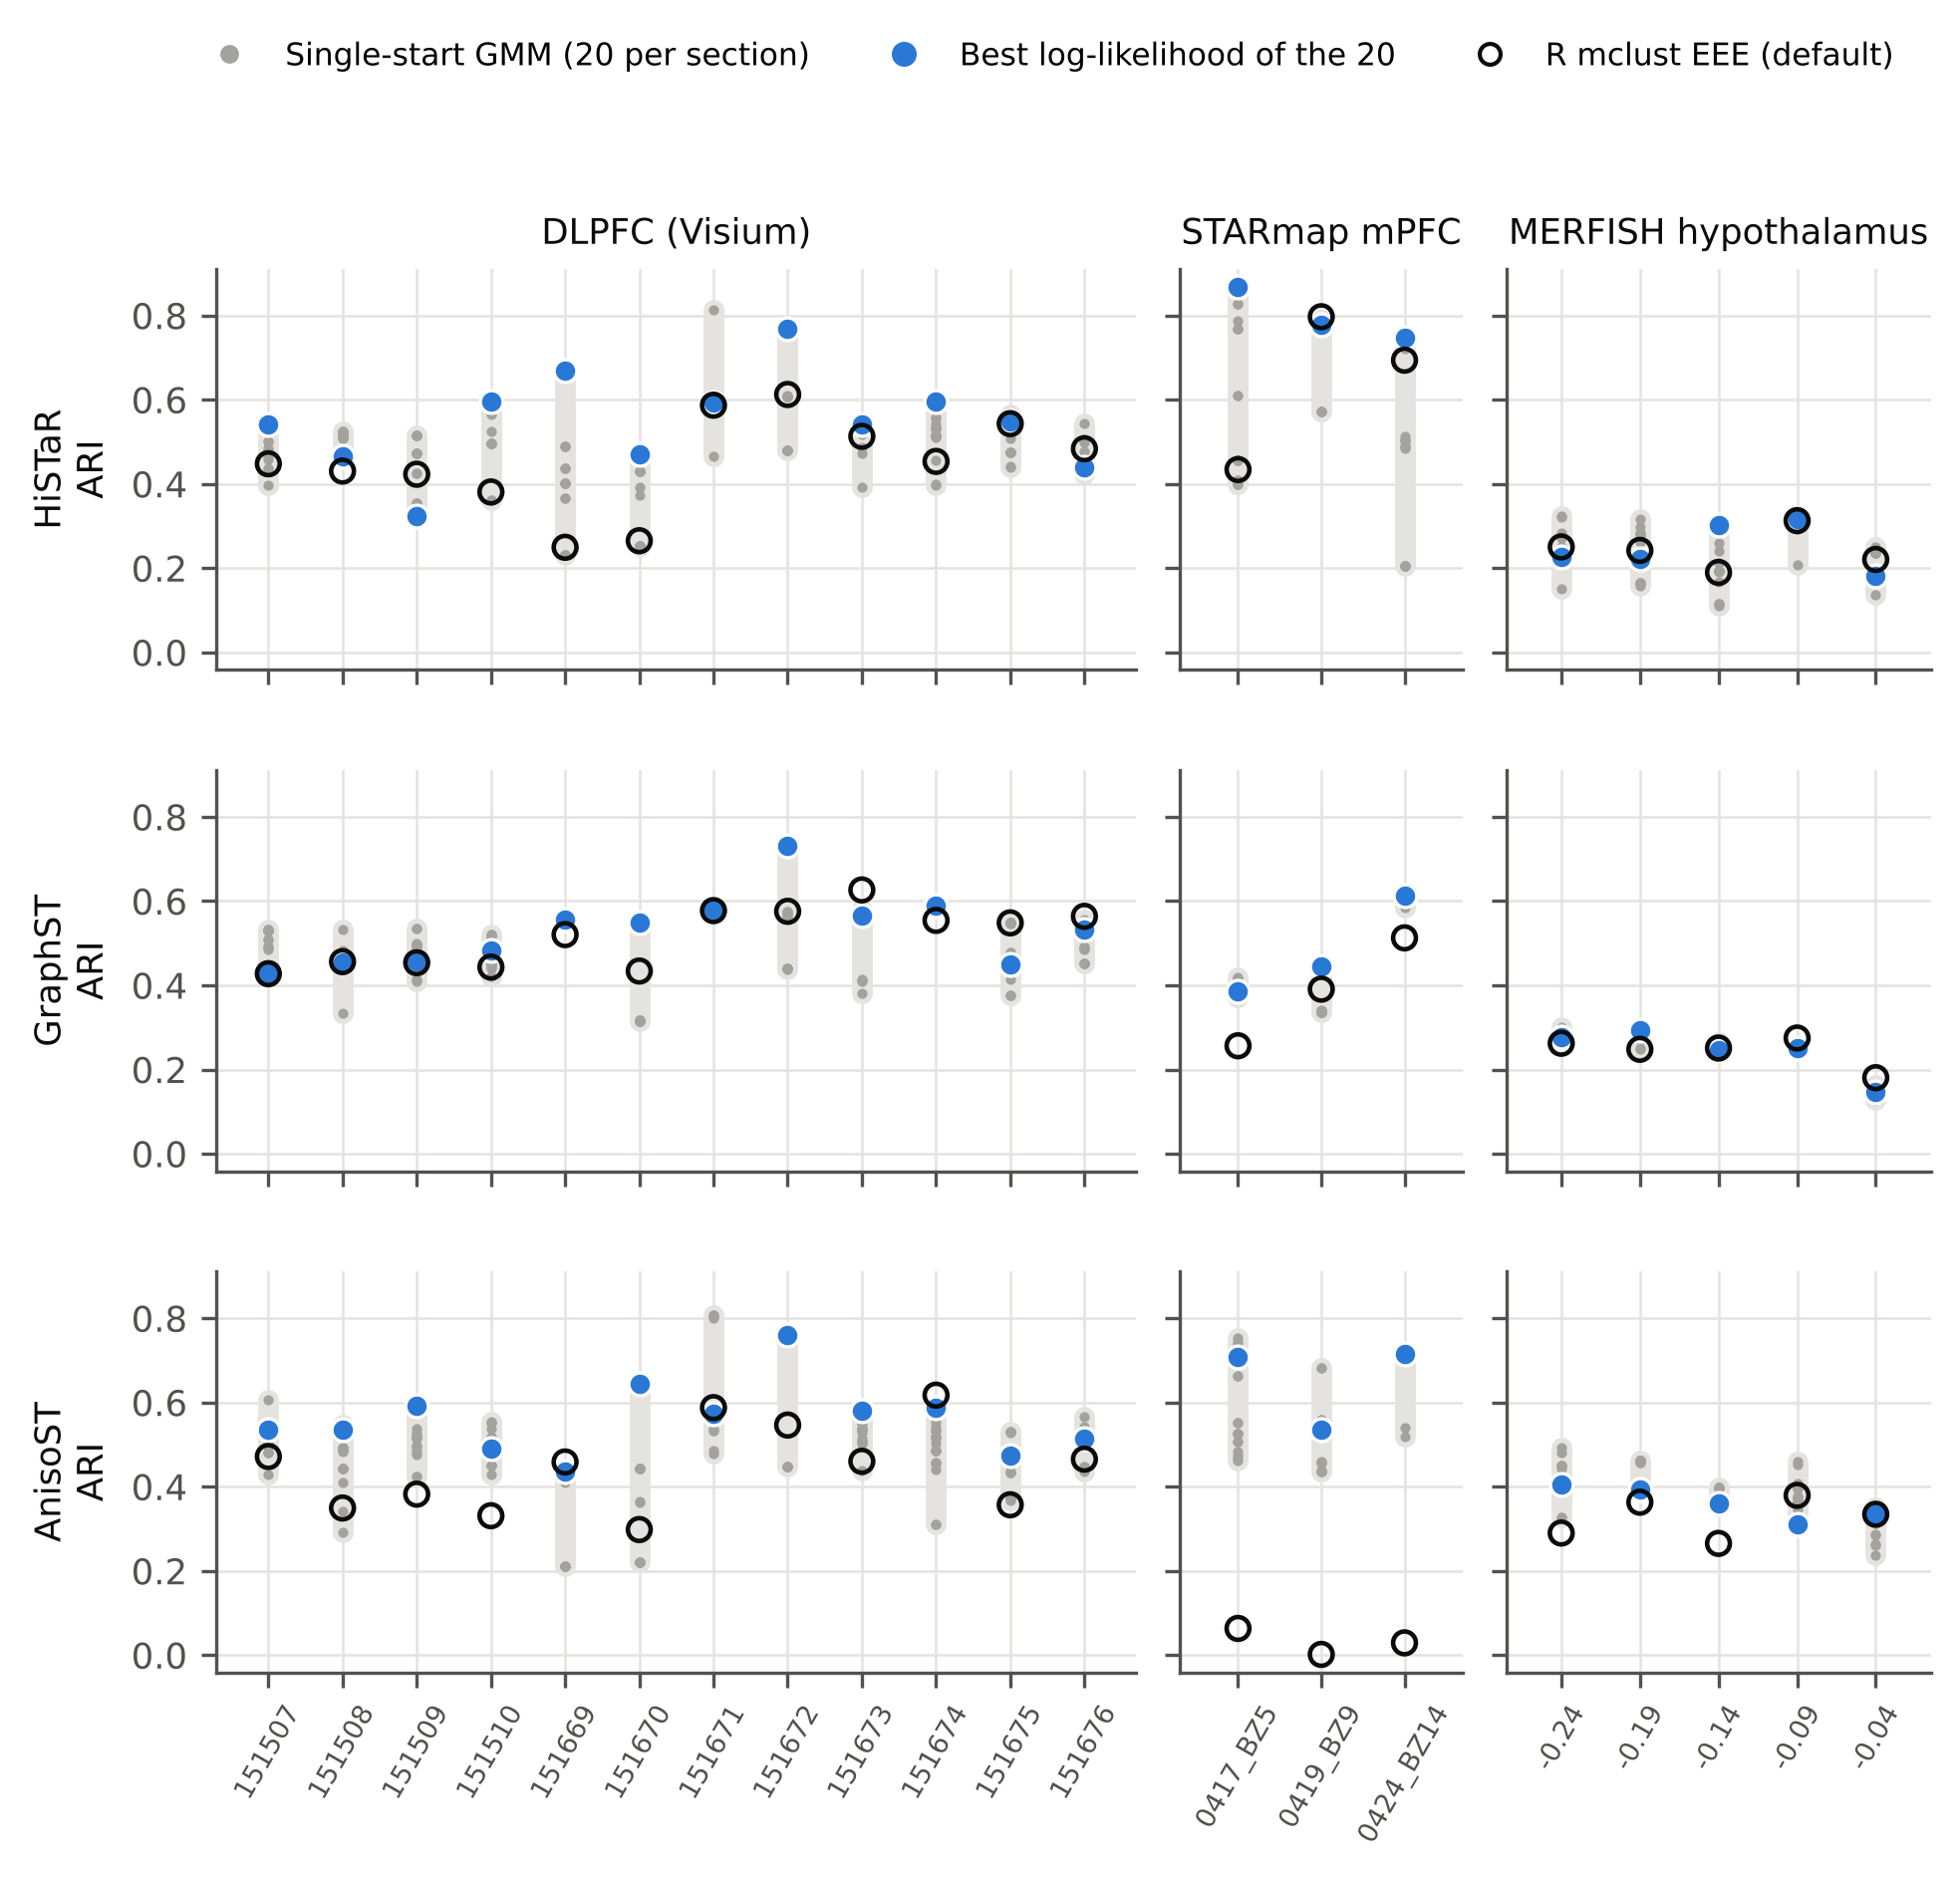
\includegraphics[width=0.9\linewidth,height=0.78\textheight,keepaspectratio]{v2_fig1_lottery.png}
\caption*{\textbf{Supplementary Figure S1.} Per-section clustering lottery for HiSTaR, GraphST and AnisoST: ARI of 20 single-start fits of one fixed embedding (grey), the best-likelihood fit (blue) and R mclust with default settings (open circle).}
\end{figure}

\begin{figure}[H]\centering
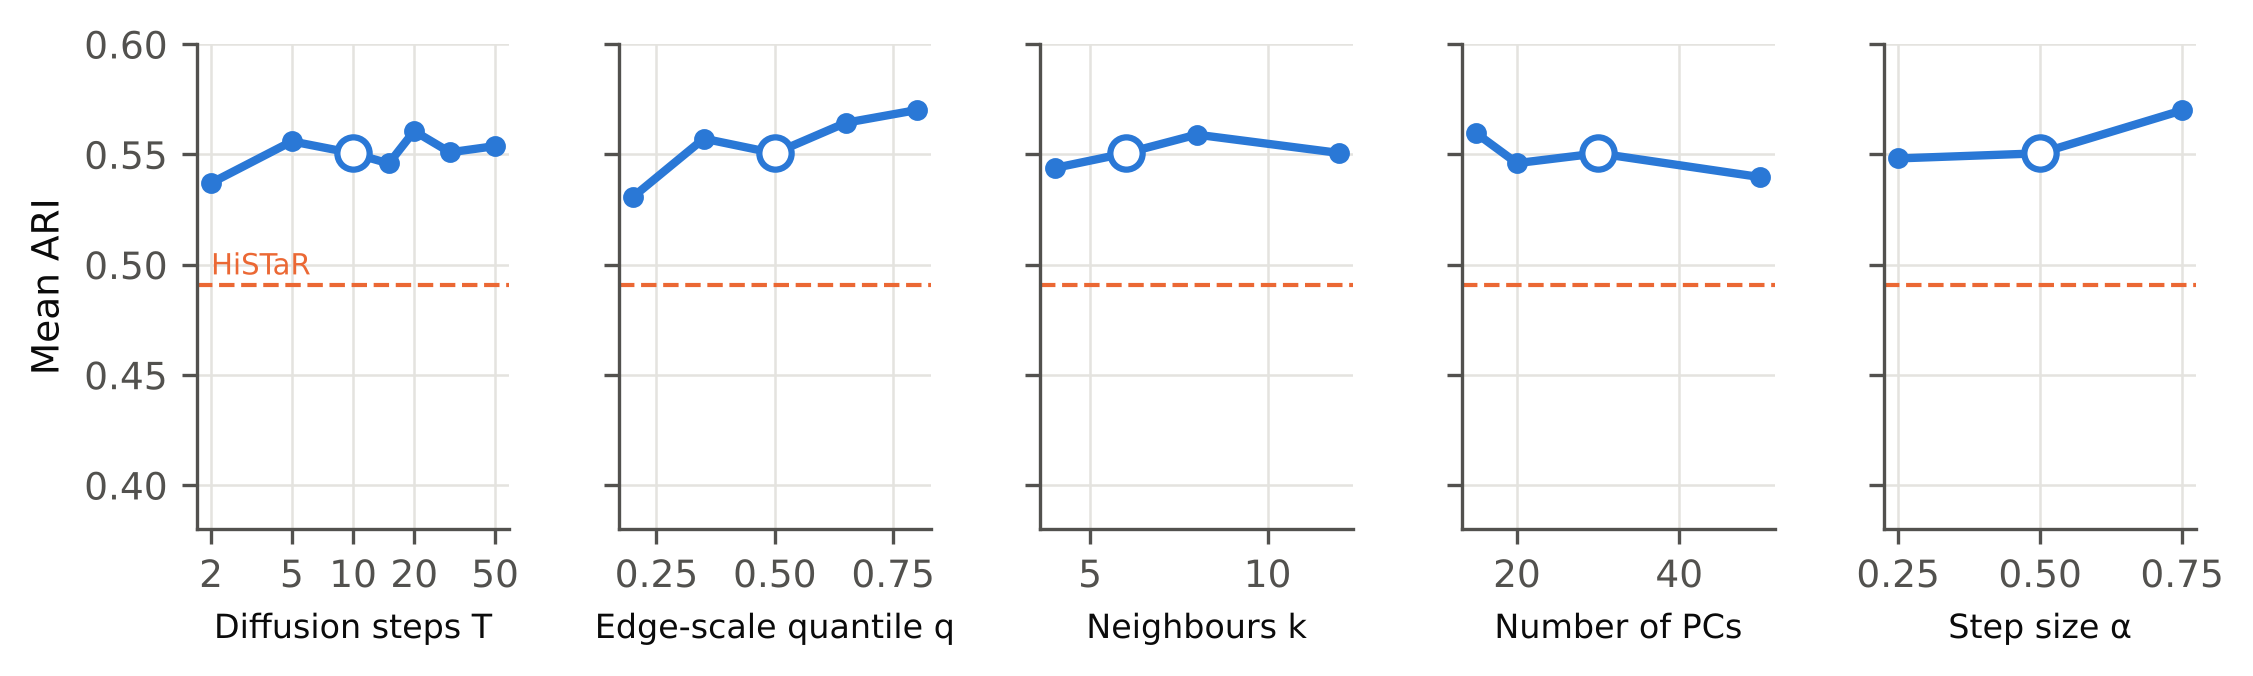
\includegraphics[width=0.9\linewidth,height=0.78\textheight,keepaspectratio]{fig3_sensitivity.png}
\caption*{\textbf{Supplementary Figure S2.} Sensitivity of the training-free baseline on DLPFC to one hyper-parameter at a time (open circle: default).}
\end{figure}

\begin{figure}[H]\centering
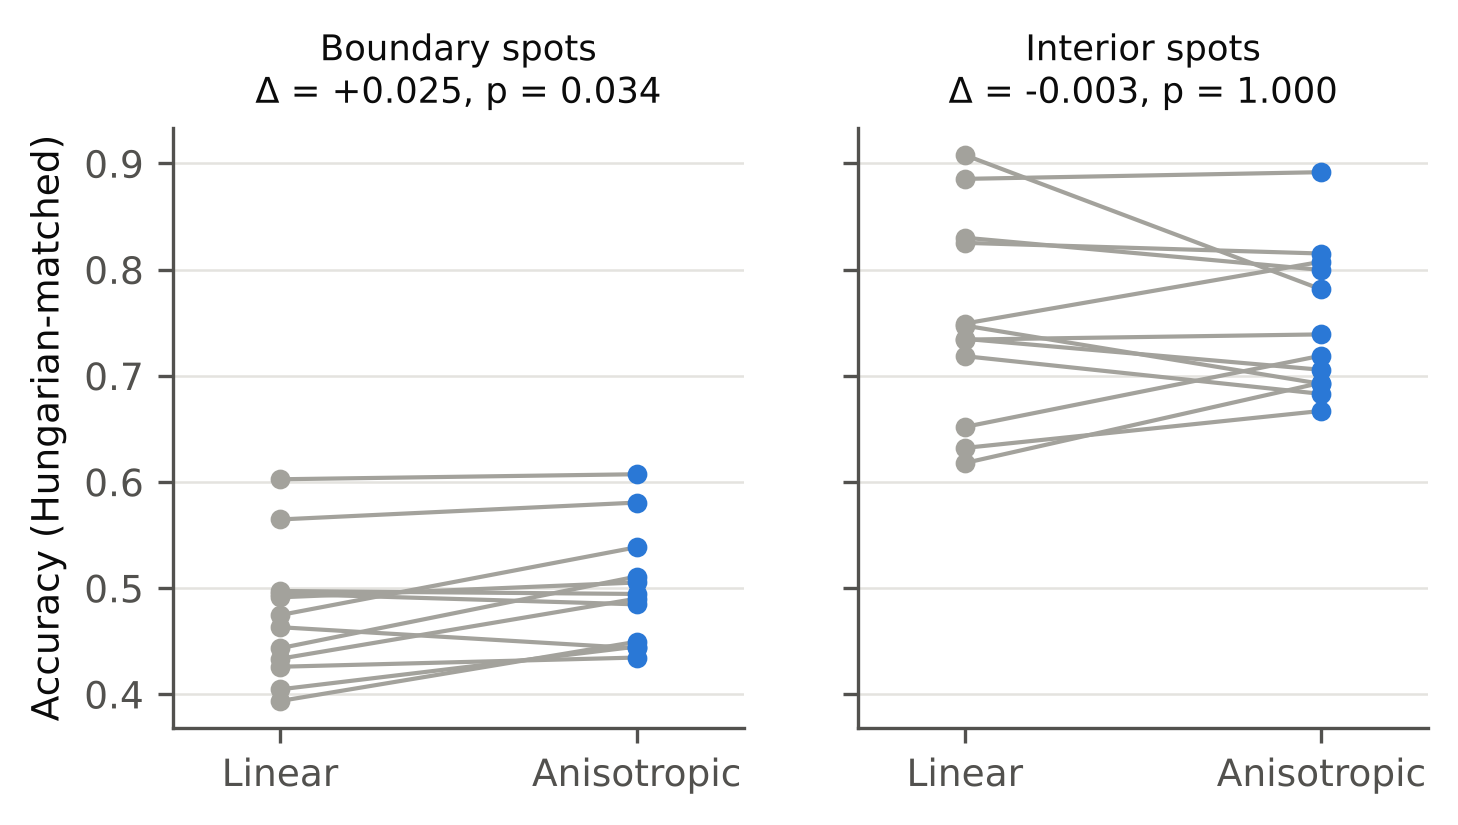
\includegraphics[width=0.9\linewidth,height=0.78\textheight,keepaspectratio]{fig4_boundary.png}
\caption*{\textbf{Supplementary Figure S3.} Accuracy on spots at layer boundaries and in layer interiors on DLPFC, linear versus edge-preserving diffusion.}
\end{figure}

\end{document}
